%%%%%%%%%%%%%%%%%%%%%%%%%%%%%%%%%%%%%%%%%%%%%%%%%%%%%%%%%%%%%%%%%%%%%%%%%%%%%%%%%%%%
% Template for STAT 548 Qualifying Paper Report
% Author: Ben Bloem-Reddy <benbr@stat.ubc.ca>
% Revised: Daniel J. McDonald <daniel@stat.ubc.ca>
% Date: 26 August 2024
%%%%%%%%%%%%%%%%%%%%%%%%%%%%%%%%%%%%%%%%%%%%%%%%%%%%%%%%%%%%%%%%%%%%%%%%%%%%%%%%%%%%

% Note: You will get an empty bibliography warning when compiling until you include a citation.

\documentclass[12pt]{article}
\usepackage[commenters={JZ,DJM}]{shortex} % replace OA with your initials
\usepackage[round]{natbib}
\usepackage[margin=2.5cm]{geometry}
\newcommand{\email}[1]{\href{mailto:#1}{#1}}

% minor adjustments to ShorTeX
\let\argmin\relax\DeclareMathOperator*{\argmin}{argmin}
\let\argmax\relax\DeclareMathOperator*{\argmax}{argmax}
\DeclareMathOperator*{\minimize}{minimize}
\DeclareMathOperator*{\maximize}{maximize}
\DeclareMathOperator{\subjto}{\ \text{subject to}\ }
\renewcommand{\top}{\mathsf{T}}
\renewcommand{\d}{\mathsf{d}}

\graphicspath{{fig/}}



%%%%%%%%%%%%%%%%%%%%%%%%%%%%%%%%%%%%%%%%%%%%%%%%%%%%%%%%%%%%%%%%%%%%%%%%%%%%%%%%%

% your title/author/date information go here
\title{STAT 548 Qualifying Paper Report DRAFT} % replace with your title, a meaningful title
\author{Justin J. Zhang} % replace with your name
\date{\today} % replace with your submission date


% start of document
\begin{document}
\maketitle

  \section{Summary of Paper}
    As the world moves forward from the Coronavirus pandemic, the question for epidemiologists and policy makers is how to 
    best prevent the spread of future novel viruses. A major step towards epidemic prevention is the accurate statistical 
    modelling of epidemic growth. Parag et al. (2022), henceforth denoted PTD, aim to tackle this problem by examining 
    two popular statistics of epidemic growth: the instantaneous reproduction number, $R_t$, 
    and the instantaneous growth rate, $r_t$. For a long time, $R_t$ has been the preeminent statistic for health professionals,
    as it explicity shows when an epidemic is growing ($R_t > 1$). However, it requires model assumptions on infection time, which
    at best induces model error, and at worst (i.e. misspecification) incorrectly predicts epidemic growth, which has drastic effects
    on real-world policy, and therefore actual lives. Sceptics argue $r_t$ is a better statistic as it does not require explicit
    model assumptions (Pellis et al., 2021) and is therefore more accurate at prediction. Under suitable distributional assumptions, 
    there is a bijective link betweeen the estimates (Wallinga \& Lipsitch, 2007). Morevover, PTD show that there is an even stronger relationship 
    between $R_t, r_t$ estimates that does not rely on model assumptions, proving that $r_t$ has implicit assumptions. 
    Ultimately, PTD try to reframe the question from ``which statistic is better?" to ``how can we use these statistics
    along with other metrics \textit{in tandem} to drive our epidemic decision making?" 
    This section covers the relevant theory and methods behind these statistics, the main contributions from PTD, 
    and the limitations in both the paper and epidemic modelling in general.

    \subsection{Relevant Theory}
      To start, we define notation. Let $t= 1,2,\dots$ be a sequence of discretized time-steps, which in PTD
      represents days. Let $I_t$ denote the $\textit{incidence of infection}$ (denoted as incidence) at time $t$, which is the number of new infections.
      Call $\{I_1,\dots,I_T\}$ the $\textit {incidence curve}$. 
      Let $\{w_j\}_{j=0}^\infty$ be the $\textit{generation time distribution}$, (Cori et al., 2013), so that $w_j$ denotes 
      the probability mass that an infected individual will generate a secondary infection in exactly $j$ days. \\
    
      The $\textit{instantaneous reproduction number}$, $R_t$, measures the mean number of secondary infections generated from each
      infected individual at time $t$, 
      with a value greater than 1 indicating a growing epidemic. The renewal model (Fraser, 2007) 
      in \cref{eq: Rt} is used to estimate $\hat{R}_t$. 
      It first computes the $\textit{total infectiousness } \Lambda_t$, 
      the number of new infections at time $t$ caused by previous incidences with respect to the generation time distribution. 
      $R_t$ is then the multiplier of $\Lambda_t$ to achieve the expected incidence number at time $t$, hence the 
      \textit{instantaneous} repreduction rate. 
      $\hat{R}_t$ is estimated from observed infections over a period $t = 1,2,\dots,T$ in terms of a specific distribution for 
      the generation time distribution using Bayesian estimation. The prior $\pi(R_t)$ is generally assumed to be from
      gamma distribution, and the likelihood $f(I_t \ | \ I_{t-1},\dots,I_1, w, R_t)$ assumed to be Poisson distributed. 
      The posterior $\pi(R_t \ | \ I_{t-1},\dots,I_1, w, I_t)$ is then derived to also be a gamma distribution, 
      and $\hat{R}_t$ is estimated based on observed incidence (Cori et al., 2013 and appendix).

      \begin{equation} \label{eq: Rt}
        \mathbb{E}(I_t) = \Lambda_t R_t, \qquad \Lambda_t = \sum_{j = 1}^{t - 1} I_{t - j} w_j \implies R_t =
         \frac{\mathbb{E}(I_t)}{\sum_{j = 1}^{t - 1} I_{t - j} w_j}
      \end{equation}

      While $R_t$ has been a mainstream measure of infectiousness for decades, it requires distributional assumptions 
      through $\{w_j\}_{j=0}^\infty$ to estimate, which complicates interpretation and accuracy (Pellis et al., 2021). 
      Accordingly, the \textit{instantaneous growth rate}, 
      $r_t$, has increased in popularity recently due its lack of distributional assumptions. $r_t$ is derived directly from
      the incidence curve, along with a smooth (log-differentiable) function $\mathbb{S}_t$, as seen in the left side of 
      \cref{eq: rt}. However, the choice of $\mathbb{S}_t$ is itself a sort of assumption as shown later.
      \begin{equation} \label{eq: rt}
        r_t = \frac{\d \log{\mathbb{S}_t}}{\d t}, \qquad S_t = \sum_{j = (1 - m)/2}^{(m  - 1)/2} I_{t + j}\alpha_j
      \end{equation}
      An example of a smoothing function is an interpolating spline between the incidences. PTD champion the
      usage of the \textit{Savitsky-Golay} (SG) filter, a local interpolation method. A SG filter of dimension $m$, with 
      $m$ odd, given in the right side of \cref{eq: rt}, performs polynomial interpolation of degree $p$, with $p \leq m$, on a 
      moving window $t - \frac{1 - m}{2}, \dots, t + \frac{m  - 1}{2}$. It derives the coefficients 
      $\alpha_{(1 - m)/2},\dots,\alpha_{(m  - 1)/2}$ for each window by least squares estimation or using a 
      pre-determined property (ex. standard moving average filter sets $\alpha_j = \frac{1}{m}$ for each $j$). The 
      derivative is then taken with respect to the fitted polynomials. \\
      
      Though no model is used, $\hat{r}_t$ is still considered an estimate in terms of a given smoothing function, which shows that 
      the choice of $\mathbb{S}$ functions as a sort of assumption. 
      
      Under the assumption of $\{w_j\}_{j=0}^\infty$ for $r_t$ there is an explicit link between $\hat{r}_t$ 
      and $\hat{R}_t$ using its moment generating function $\mathbb{M}_w$
      (Wallinga \& Lipsitch, 2007). The general formulation, called the Lotka-Euler equation,
      as well a specfic instance where $w_j$ is taken from a 
      $Gamma(\alpha, \beta)$ distribution is given in \cref{eq: rt-Rt}. The equation is derived by further assuming 
      exponential growth (or decay) for the incidence at a rate of $\hat{r}_t$, that is $I_t = I_{t-j} e^{j \hat{r}_{t - j}}$
      (appendix). This gives a bijective relation to obtain $\hat{r}_t$ directly from an estimate of $\hat{R}_t$. 
      \begin{equation} \label{eq: rt-Rt}
        \hat{R}_t \mathbb{M}_w(-\hat{r}_t) = 1, \qquad \hat{r}_t = \beta(\hat{R}_t^{\frac{1}{\alpha}} - 1)
      \end{equation}

    \subsection{Main Contributions}
      Though this estimate $\hat{r}_t$ is model-dependent, PTD show that there is additionally a non model-dependent connection between 
      $\hat{R}_t, \hat{r}_t$ that refutes the notion from (Pellis et al., 2021), (Dushoff \& Park, 2021) and others that
      the distributional assumptions on $\hat{R}_t$ minimize its usage.
      The novelty PTD introduce is to prove the connection between $\hat{R}_t, \hat{r}_t$, and determine their respective advantages and disadvantages. 
      This is illustrated through a case study on the epidemic
      growth of the Ebola virus in West Africa (Van Kerkhove et al., 2015). $\hat{R}_t$ is estimated through the \textit{Epifilter} 
      package in R, but section 3 will reproduce the simulations using \textit{rtestim}. $\hat{r}_t$ is estimated in three ways: 
      directly using SG filters as in \cref{eq: rt}, directly using total infectiousness $\Lambda_t$ as a smoothing function, and 
      from $\hat{R}_t$ using \cref{eq: rt-Rt}. All models estimate $R_t$ and $r_t$ with low prediction error, though $(\hat{r}_t \ |\ S_t) < r_t$
      consistently when $I_t$ is small. This is because the fitted spline will further flatten the already low incidence rates, 
      an issue more pronounced at low absolute values. The predicted $\hat{r}_t \ |\ S_t$ must by right shifted $\frac{m-1}{2}$
      days as it requires knowledge of incidence at time $t + \frac{m-1}{2}$ and so the local spline fitted for $S_t$ is used
      to predict growth rate $\hat{r}_{t + (m-1)/2}$. Likewise,  $\hat{r}_t \ |\ \Lambda_t$ must be left shifted $\frac{m-1}{2}$
      days as it requires knowledge of the incidences at $t - m,\dots,t$ to estimate growth rate $\hat{r}_{t - (m - 1)/2}$
      (estimation is on midpoint). Generally, $\Lambda_t$ actually requires the incidences starting at time 1, but the 
      probability for primary transmission before $t - m$ is near 0.\\

      The estimation of $r_t$ using total infectiousness and SG filter as smoothing functions shows the explicit link between
      the model assumptions and choice of smoothing function. In fact PTD show $\Lambda_{t+\tau}$ is approximately equal to $S_t$ 
      for $\tau \approx \mathbb{E}(w)$. Both are functions of the daily incidence, and so under correct model specification the
      estimated coeffcients $\alpha_j$ determine it's own distribution. That is,
      \begin{equation} \label{lambda SG}
        w_j \approx \alpha_{\tau - j} \implies 
        \Lambda_{t+\tau} = \sum_{j = 1}^{t + \tau - 1} I_{t + \tau - j}w_j  
        \approx \sum_{j = 1}^{2\tau - 1} I_{t + \tau - j}\alpha_{\tau -j}
        \approx \sum_{j = 1 - \tau}^{\tau - 1} I_{t - j} \alpha_{-j}
        = \sum_{j = 1 - \tau}^{\tau - 1} I_{t + j} \alpha_{j}
      \end{equation}
      $w_j$ will be generally near 0 for $j > 2\tau = 2\mathbb{E}(w)$ (this can be shown for example if $w$ follows poisson). 
      Setting $m = 2\tau - 1$ will equate the final equality in \cref{lambda SG} with the SG filter in \cref{eq: rt}.
      \cref{lambda SG} shows that generation time distirbution is functionally a smoothing filter through $\Lambda_t$, meaning
      the assumptions on $\Lambda_t$ are used to compute both $\hat{R}_t, \hat{r}_t$ .This linkes
      $R_t$ and $r_t$ with a stronger result than \cref{eq: rt-Rt} as this relation connects a non-model dependent $\hat{r}_t$ with $\hat{R}_t$, 
      showing that $\hat{r}_t$ has underlying implicit model assumptions, 
      which refutes a major advantage it has over $\hat{R}_t$ (Pellis et al., 2021). 
      In this relation, the coefficients $\alpha_j$ form an arbitrary kernel for each $S_t$ that is similar to the generation time
      distribution kernel. It is worthwile to mention that PTD only show this relation for the SG filter as a smoothing funciton, not for smoothing
      functions in general.
      Nonetheless, Parag et al. (2022) argue there are benefits to using both statistics in conjuction to 
      model epidemic growth and inform public policy. \\

      One significant benefit of estimating $r_t$ is performance when the generation time distirbution 
      is misspecified. $\hat{R}_t$ is derived immediately from $w$ and so naturally has high bias under misspecification, 
      however using \cref{eq: rt-Rt} to compute $\hat{r}_t$ from the poorly estimated $\hat{R}_t$ 
      still recovers an estimate of $r_t$ with low bias. 
      Under good model specification, PTD argue $\hat{R}_t$ is a more infomrative estimate of epidemic growth 
      since $\hat{r}_t$ is estimated from it. However, under reasonable assumptions where both estimates have low error, 
      the two statistics can and should be used in conjunction to inform health policy. $\hat{R}_t$ quantifies the number of
      secondary transmissions that need to be prevented on average to slow the pandemic, which is a determining factor in 
      epidemic control policy and vaccine coverage. $\hat{r}_t$ measures the speed of epidemic growth, 
      and gives metrics such as doubling time, which is a determining factor in intervention planning (ex. lockdowns). 
      Ultimately, PTD argue that \textit{both} $\hat{R}_t, \hat{r}_t$ are essential to understanding and 
      implmenting informed policy for epidemics, which is of utmost importance to society as a whole.

    \subsection{Limitations}
      There are a number of limitations to the work in Parag et. al (2022), both in there analysis comparing $\hat{R}_t, \hat{r}_t$
      and its applicability to accurately model epidemics. Incidence data, denoted as the time when an individual 
      first contracts the disease is almost always earlier than the report date. Thus 
      incidence values are right censored estimates, requiring future case numbers and incubation times,
      as well as other factors like susceptibility rates. In some cases, it will also be left censored if baseline infections
      from the start of an epidemic are not known (Fraser, 2007) due to epidemiologists not understanding the severity. 
      Furthermore, a decent percentage of incidences are never reported,
      and so the true incidence is impossible to know. This adds a layer of data-dependent irreducible variance to 
      $\hat{R}_t, \hat{r}_t$, which can have a multiplicative effect on total error, an issue PTD never 
      mention ways to mitigate. One possible solution (Comiskey et al., 2021) is to model the distribution of incubation time, 
      say $\{\xi_i\}_{i=1}^\infty$, say with gamma distribution and use observed cases $C_t$ to back-calculate incidence, 
      $\hat{I}_t = \sum_{i=0}^\infty \xi_i C_{t+i}$ . 
      This hopes that the additional variance from an extra layer of prediction is less than the reduction in variance on the main
      model (error due to unreported cases is still unavoidable). Another issue
      that is not addressed is the case of a single secondary infection coming from numerous primary sources, a common issue when
      larger groups of people hang out together. It is ambiguous how this should be attributed, whether it should be equal
      percentages to each source, attributed to a single transmitter only, or attributed in whole to each transmitter. 
      The last option means $\hat{R}_t$ will be underestimated as there is only 1 incidence that will go towards the $\Lambda_t$ 
      calculation. The first 2 options are mathematically okay, but lead to different interpretations, 
      which are not clarified in PTD.
      
      There are also outside factors to consider that would impact incidence rate and hence $R_t, r_t$. 
      The presence of singular events with high transmission possibility, for example festivals and concerts, 
      will cause a jump in daily incidence. Days and seasons with good weather will have more people outdoors, leading to higher
      incidence as well. It may be possible to include a multiplier for total infectiousness for these effects, say 
      $\Lambda_t = \lambda_t \sum_{j=1}^{t-1}I_{t - j}w_j$, where $\lambda_t > 0$ measures deviation from baseline level of human interaction 
      and can be estimated from a simple regression model. $\lambda_t$ should be so that values less than 1 correspond to a likely
      increase in infections above average (and vice versa). This is due to $\Lambda_t$ being artificially lowered, 
      and keeping the distributional assumptions on $\mathbb{E}(I_t)$ the same, 
      $R_t$ will be higher than the expeceted rate without accounting for outside factors. Alternatively, the times series
      $I_1,...,I_t$ can incorporate these outside factors through various effect variables. This would then increase or decrease
      $\mathbb{E}(I_t)$ from benchmark values (i.e. no effect) accordingly, and in turn decrease or increase $\hat{R}_t$.
      PTD account for seasonal differences in their example, but no other outside influence addressed, though 
      they off-handedly mention ``contextual information" as something that is needed. There are also human-influenced outside
      factors that can shift the entire reproduction rate curve, the most prevalent being vaccine mandates and quarantines. 
      There is a related statistic (not mentioned by PTD), 
      the \textit{case reproduction number}, $R^x_t$, which measures the average number of secondary infections over a lifetime.
      This statistic will implicitly account for these changes, but can only be back-calculated as a
      retrospective statistic, as it requires future incidence numbers (Cori et al. 2013). There is also the 
      \textit{Susceptible-Infectious-Recovered} model that groups people into these three categories, but it is often an
      oversimplication of true epidemic dynamics (Lloyd, 2009).  (TIE THIS BACK TO PAPER)

      
      Conceptually, the largest limitation is that PTD never discuss \textit{how} to use $\hat{R}_t, \hat{r}_t$ together to
      understand epidemic dynamics. For a paper who's primary objectives are to clarify the understanding of these statistics, 
      there is not any concrete applications beyond ``use both". Furthermore, most of the theory is hand-waved, which is okay
      because they reference the background papers, but is difficult for readers to both understand their assumptions, and follow
      their logic. In summary, PTD do a sufficient job to compare $\hat{R}_t, \hat{r}_t$ and refute the thought that the lack
      of distributional assumptions in $\hat{r}_t$ is an inherent advantge, but beyond that they have not developed any novel 
      methods or ideas that can be applied to real-world epidemiological modelling, which is subpar for an applied paper. 

  \section{Mini-Proposals}
      In the previous section, we discussed PTD's claim that the smoothing function assumed to estimate $r_t$ is itself an implicit
      distributional assumption, which refutes claims that $r_t$ is a better statistic to measure epidemics (Pellis et al., 2021). 
      The logical next step is to consider whether we can still estimate $r_t$ without the use of any explicit smoothing functions.
      In this section we propose a method to smooth the parameters $r = (r_1,\dots,r_T)$ directly rather then smoothing the
      incidence itself (ex. SG filter), thereby estimating $\hat{r} = (\hat{r}_1,\dots,\hat{r}_T)$ without functional assumptions. 

      Recall that the incidence is assumed to come from a Poisson parameter. Previously in the renewal model we took the rate as
      $\Lambda_t R_t$ (Cori et al., 2013), however since we are no longer applying distributional assumptions we simply
      use exponential growth, that is $I_t|I_{t-1} \sim \text{Poisson}(I_{t - 1}e^{r_t})$ where the parameter of interest is $r_t$.
      This is a \textit{Poisson many means model} where each observation $I_t$ has a different rate parameter. We also have 
      simplifying assumption of independence, which likely does not hold because $I_t$ is explicitly dependent on $I_{t - 1}$.
      The first naive method of estimation we would consider is to simply take the MLE
      \begin{align} \label{rt: MLE}
          (\hat{r}_1^{MLE},\dots,\hat{r}_T^{MLE}) &= \argmax{r \in \mathbb{R}^T} \mathcal{L}(r_1,\dots,r_T ; I_1,\dots,I_T) \\
          &= \argmax{r \in \mathbb{R}^T} \prod_{t = 2}^T \frac{(I_{t - 1}e^{r_t})^{I_t} e^{-I_{t - 1}e^{r_t}}}{I_t!} \\
          &= \argmin{r \in \mathbb{R}^T} \sum_{t = 2}^T -[I_t(\log{I_{t - 1}} + r_t) - I_{t - 1}e^{r_t}]
      \end{align}
      Deriving in terms of each $r_t, \; t=1,\dots,T$ and setting to 0 gives a set of solutions \\ 
      $\hat{r}_t^{MLE} = \log{I_t} - \log{I_{t - 1}}$. Note that for this paper, we assume that 
      $I_t > 0$ by increasing each $I_t$ by some small tolerance $\epsilon$ (say $\epsilon = 1$) so we can safely take logarithms.

      The MLE under Poisson assumption gives an unbiased estimator w.r.t. incidence, that is $E(I_{t - 1}e^{\hat{r}_t} | I_t) = I_t$. 
      However, since we have assumed independence, the risk of this set of estimator $\hat{r}^{MLE}$ under square error is
      \begin{align}
        R(I_{-1}\hat{r}^{MLE}, I) = \sum_{t = 2}^T \mathbb{E}(I_t - I_{t - 1}e^{r_t})^2 = \sum_{t = 2}^T \text{Var}(I_t) = \sum_{t = 2}^T I_{t - 1}e^{r_t}
      \end{align}

      Here, $I_{-1}$ is the incidence vector shifted 1 day to the left, so that ${I_{-1}}_t$ matches $I_{t + 1}$. 
      Accordingly, the loss function sums from $t = 2$ as $t = 0$ data is assumed unavailable.
      Since incidence will be non-negative for non-trivial epidemics, and similarly growth rate will not be strictly negative, as $T \to \infty$, 
      this risk function will blow up to infinity. This is because each $\hat{r}_t^{MLE}$ is fit individually, 
      which gives unbiasedness but increases variance for $r^{MLE}$ as a whole. Moreover, based on the incidence curve, we can very well get $\hat{r}_t^{MLE}$ jumping around, 
      leading to an incredibly unsmooth estimator, as shown in (FIGURE). 
      
      As such, our goal is decrease the estimator variance by inducing some (hopefully small) level of bias. 
      Our proposed method is to add a smoothing function on the parameters themselves. This is opposed to 
      \cref{eq: rt} which smooths the data. The method is analogous to the \textit{rtestim} method of estimating $R_t$ (Liu et al., 2024).
      Functionally, we are applying a penalty on the differences in growth rates and adding it to the Poisson loss
      from \cref{rt: MLE}. We get the smoothed estimator in \cref{rt: smooth}
      \begin{align} \label{rt: smooth}
          (\hat{r}_1^{lambda},\dots,\hat{r}_T^{lambda}) &= \argmin{r \in \mathbb{R}^T} \sum_{t = 2}^T [I_{t - 1}e^{r_t} - I_t(\log{I_{t - 1}} + r_t)] \\
          &\qquad + \lambda_1 \sum_{t = 2}^T e^{(r_t - r_{t - 1})^2} + \lambda_2 \sum_{t = 3}^T e^{(r_t - 2r_{t - 1} + r_{t -2})^2}
      \end{align}

      The corresponding derivative of this objective function $\ell$ in \cref{rt: deriv} is not directly solvable for $\hat{r}_t^{lambda}$, 
      but note that the second derivative is strictly positive on an assumed sample space (appendix) and so $r\hat{r}_t^{lambda}$ can be solved
      with pre-existing convex optimization methods. 

      \begin{equation} \label{rt: deriv}
          \frac{\partial \ell(r; I)}{\partial r_t} = I_{t - 1}e^{r_t} - I_t + e^{(r_t - r_{t - 1})^2} (2(r_t - r_{t - 1})) 
          - e^{(r_{t+1} - r_{t})^2} (2(r_{t+1} - r_{t}))
      \end{equation}

      At a high level, the solution to \cref{rt: smooth} will smooth the estimated parameters in 2 ways. The first penalty term $e^{(r_t - r_{t - 1})^2}$ controls
      the magnitude of the first difference in growth rates $r_t - r_{t - 1}$, which ensures there are no big jumps in growth rate between days. 
      The second penalty term $e^{(r_t - 2r_{t - 1} + 2r_{t - 2})^2}$ controls
      the magnitude of the second differences $r_t - 2r_{t - 1} + 2r_{t - 2} = (r_t - r_{t - 1}) - (r_{t - 1} - r_{t - 2})$, 
      which ensures that concavity is not constantly changing. There is no practical benefit to taking exponents, but is is done to maintain the same scale 
      for growth rate as in the Poisson rate. Similarly, we could take absolute differences rather than squared differences. $\lambda_1, \lambda_2$ are 
      hyperparameters that would be tuned using cross-validation when modelling $\hat{r}_t$.

      As a motivating example, we consider a single simulated epidemic, under the same conditions as \cref{fig: paper}. The figures show the estimators (in blue)
      of the true growth rate (in black). Plot a) models $\hat{r}^{MLE}$ using \cref{rt: MLE}, plot b) models $\hat{r}$ with first difference penalized, 
      and plot c) models $\hat{r}$ with first and second differences penalized as in \cref{rt: smooth}. From the plots we can see that the desired properties 
      we mentioned above are present as first and second differences successfully control frequent changes in magnitude and concavity respectively, 
      leading to a smooth estimator. It turns out the MSE of this estimator is lower than the MSE using the SG filter in \cref{fig: paper}.

      \begin{figure}[h]
        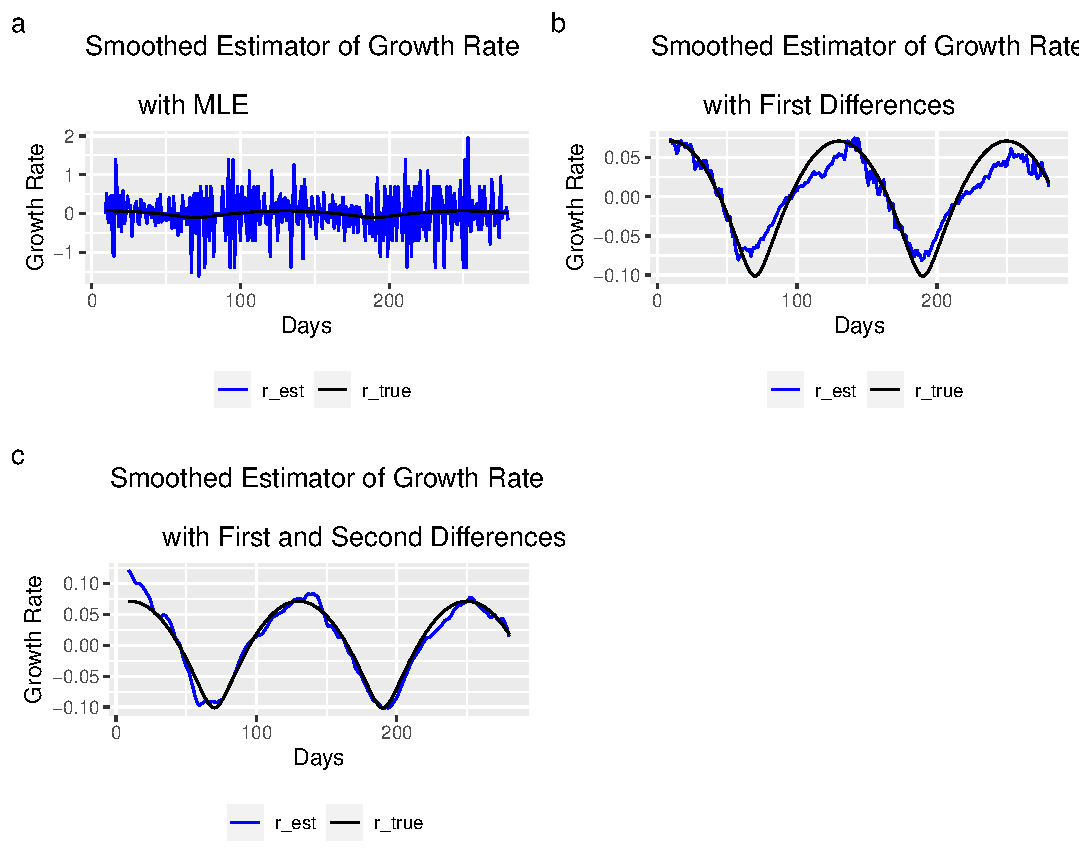
\includegraphics[width = \linewidth]{estimate_growthrate.pdf}
        \caption{asd}
        \label{fig: smoothrt}
      \end{figure}

      To move this proposal forward, there a couple main ideas to explore:
      \begin{enumerate}
          \item Determine the implementation details of the estimation method. Details to examine include which specific penalty function to apply and
          how to solve \cref{rt: smooth} numerically. The above proposal uses first and second differences, but it may be that penalizing higher order
          differences or only using 1 penalization term reduces MSE. There should be consideration for whether absolute differences can be used
          over squared differences as in (Liu et al., 2024) but that is a more difficult optimization to solve. The example in \cref{fig: smoothrt}
          uses R built-in \textit{optim} function, but other implementations can likely increase convergence speeds and accuracy.
          \item Compare parameter based smoothing (our method) versus data based smoothing (PTD and \cref{eq: rt}) in terms of MSE, smoothness, and 
          other statistical measures. It is also worth examining how our method does with real data, which will exhibit greater variance in incidence numbers,
          in terms of estimator smoothness. Furthermore, with noisy data, is it plausible to smooth both the data and the estimator, i.e. run our method
          on smoothed data.
          \item Consider the claims made in PTD with our new method, that does not rely on functional assumptions. Evaluate what underlying assumptions are 
          present and how they relate to the estimation of $\hat{R}_t$ as PTD do by comparing SG filter and infectiousness kernel.
      \end{enumerate}






  \section{Project Report} 
      To substantiate the findings in PTD, we will do a series of computational experiments to first verify their claims, 
      and then discover conditions under which $R_t$ and $r_t$ fail to accurately model the epidemic. Since true $R_t$ values are
      near impossible to determine from real, we use simulated epidemics. In this section, we conduct (INSET NUMBER) empirical 
      experiments to better understand model performance under various epidemic conditions. To do this, we consider the 
      following models (with generation time distribution $\text{Gamma}(2.7066, 2.7066 / 15.3)$):
      \begin{enumerate}
        \item True $R_t$ following sinusoidal curve
        \item True epidemic as above but $\hat{R}_t$ estimated using generation time distribution with $\frac{1}{3}$ to true mean
        \item True $R_t$ follwing piecewise constant
      \end{enumerate}

      To generate true (simulated) incidence and infectiousness, we iteratively compute $\Lambda_t$ from $I_{1},\dots,I_{t - 1}$ and 
      $\{w_j\}_{j=0}^\infty$, and then $I_t$ from $R_t$ and $\Lambda_t$ as in the renewal model in \cref{eq: Rt}. To estimate $\hat{R}_t$
      PTD uses \textit{EpiEstim}, a Bayesian method that estimates the posterior as in (APPENDIX) and smooths the resulting estimates.
      We will use \textit{rtestim} (Liu et al., 2024), a frequentist approach which fits a penalized spline with Poisson loss and $\ell_1$ penalty on $\log{R_t}$, and solves with proximal Newton method.
      The objective function in this optimization problem is

      \begin{equation} \label{rtestim}
        \hat{\theta} = \argmin_{\theta \in \mathbb{R}^t} \Lambda^T \exp{\theta} - I^T\theta + \lambda \Vert\ D^{k+1} \theta \Vert\_1
      \end{equation}
      Here, $\theta = \log{R}$, $\Lambda, R, I \in \mathbb{R}^t$  are the respective infectiousness, reproduction rate, and incidences across $t$ time-steps, $D$ is the divided differences matrix, and $\lambda$ is a hyperparameter that controls smoothness. 
      \textit{rtestim} tunes $\lambda$ across a grid of possible values, and $\lambda_{min}$ that minimizes cross validation error is used in the following results. 
      (Liu et al., 2024) show that \textit{rtestim} estimates $\hat{R}_t$ at least as well \textit{EpiEstim} with respect to Kullback Leibler (KL)  Divergence.

      To quantify prediction accuracy of $\hat{R}_t$ and $\hat{r}_t$, we use KL divergence and mean squared error respectively over $t = 1,\dots,T$, as shown in \cref{acc}.
      KL divergence is used as distance measure becauase it handles the non-negativity of $R_t$ and models the Poisson assumption 
      used in \textit{rtestim} and \cref{eq: Rt} (Liu et al., 2024).

      \begin{equation} \label{acc}
        D_{KL}(R, \hat{R}) = \KL(R \Vert\ \hat{R}) = \sum_{t = 1}^T \lambda_t \left( R_t \log{\frac{R_t}{\hat{R}_t}} + \hat{R}_t - R_t \right) \quad 
        D_{MSE}(r, \hat{r}) = \sum_{t = 1}^T (r_t - \hat{r}_t)^2
      \end{equation}

      For a simulated epidemic, we wish to show that $\hat{R}_t$ and $\hat{r}_t$ accurately estimate their respective rates. Moreover, we wish to substantiate PTD's claim
      that total infectiousness suffices as a smoothing filter, hence SG filters implicitly forms a SG filter.
      We take the true instantaneous reproduction rate $R_t = 1.3 + 1.2\sin{\frac{\pi t}{60}}$ and generation time distribution $\text{Gamma}(2.7066, 2.7066 / 15.3)$. 
      This reproduces the first example in PTD, with results are reported in \cref{fig: paper}. From subplots a) and b), it is clear that $\hat{R}_t$ and $\hat{r}_t$ have the shape and convey information, 
      that is $\hat{R}_t > 1 \iff \hat{r}_t > 0$ to signify when the epidemic is growing or shrinking. This is expected when we take $\hat{r}_t \ |\ \hat{R}_t$ from \cref{eq: rt-Rt}
      but it also holdds for SG filters in this case. Subplot d) shows that the left-shifted $\Lambda_t$ is approximately equal to the smoothed incidence $S_t$, 
      which in this example confirms PTD's claim. In this simulation the only assumptions we made on $\hat{r}_t$ is the use of the SG filter with moving window 
      $2\tau + 1 = 31$ time-steps and cublic spline fits, hence the smoothing function $\mathbb{S}(t)$ functionally approximates the generation time distribution.

      \begin{figure}[h]
        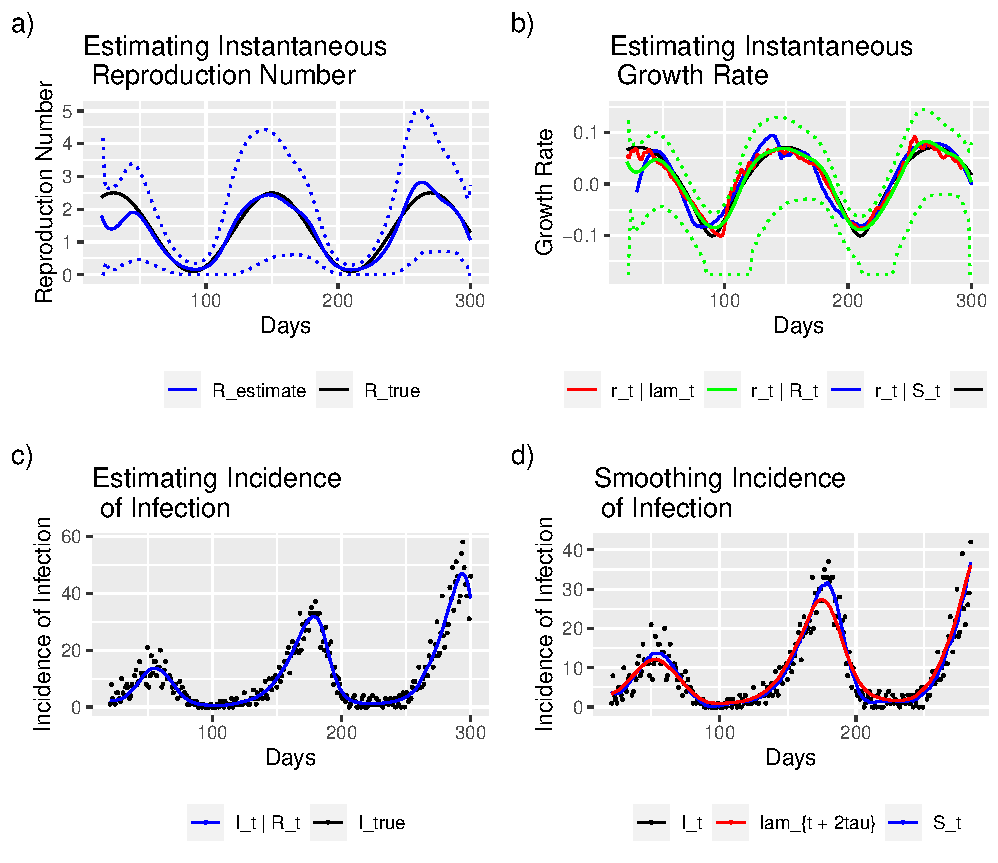
\includegraphics[width = \linewidth]{epi_paper.pdf}
        \caption{asd}
        \label{fig: paper}
      \end{figure}

      The first deviation from satisfactory conditions is to use a misspecified generation time distribution, as done in PTD. This is quite reasonable in reality as it is
      difficult to assign the generation time distribution due to not observing true incidence of infection and using cases to estimate. 
      This is specially prominent early in an epidemic when there is a lack of data to estimate the generation time distribution and basing a prior on other epidemics is risky. 
      We would assume that the estimates for $R_t$ under these conditions would be poor because $\Lambda_t$ is dependent on generation time distribution and since we are still
      using the true incidence, from \cref{eq: Rt} $\hat{R}_t$ must necessarily deviate from the true $R_t$. 
      In our case take $\{w_j^{misspec}\}_{j=0}^\infty \sim \text{Gamma}(2.7066, 2.7066 / 15.3 * 3)$, which has $\frac{1}{3}$ the expected value of the true distribution in \cref{fig: paper}. 
      In \cref{fig: misspec} we see that $\hat{R}_t$ is a very poor estimator w.r.t. KL divergence,
      However $\hat{r}_t \ |\ \hat{R}_t$, i.e.$\hat{r}_t$ derived from $\{w_j^{misspec}\}_{j=0}^\infty$ and the same (poor) $\hat{R}_t$, performs well w.r.t. MSE. 
      In fact, $D_{KL}(R, \hat{R}^{misspec}) \approx 310$ whereas $D_{KL}(R, \hat{R}) \approx 24$, an over tenfold difference, but $D_{MSE}(r, \hat{r}) \approx 0.29$ is close 
      (at least in absolute terms) to $D_{MSE}(r, \hat{r}) = 0.09$. 

      \begin{figure}[h]
        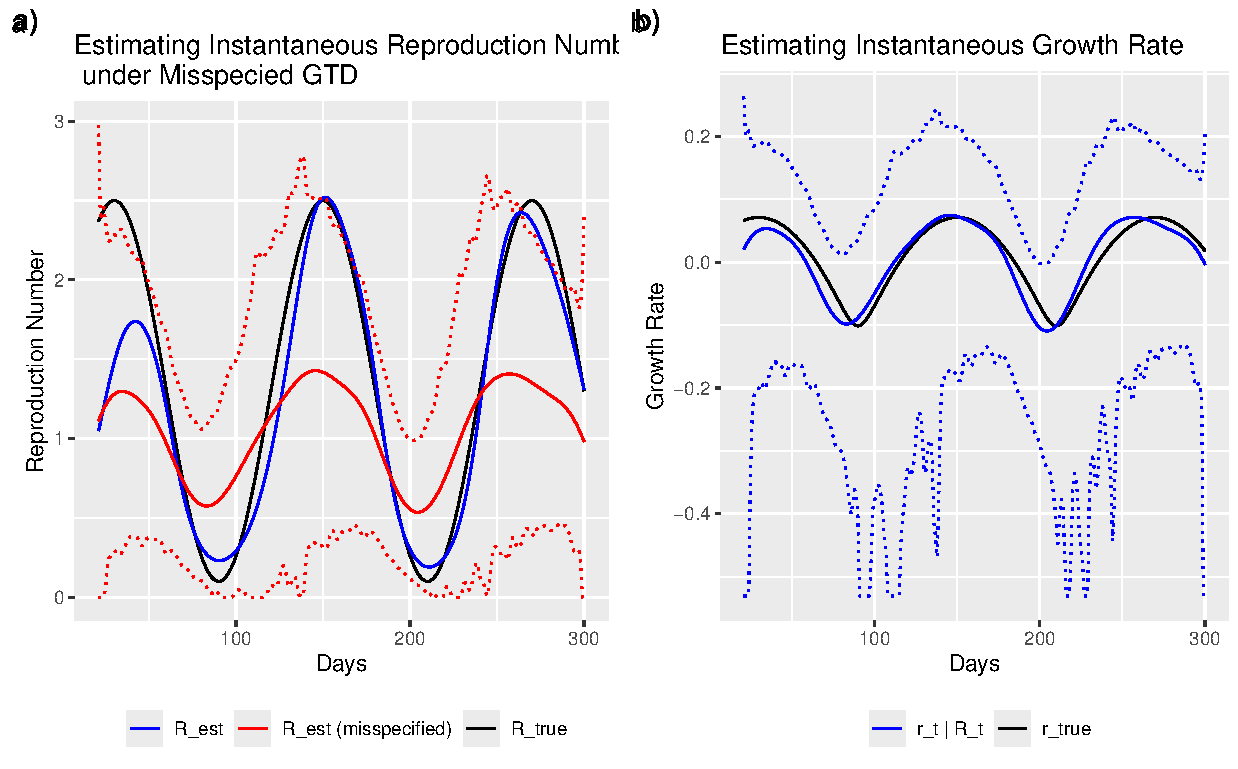
\includegraphics[width = \linewidth]{epi_misspec.pdf}
        \caption{asd}
        \label{fig: misspec}
      \end{figure}

      \newpage

      \begin{figure}[h]
        \centering
        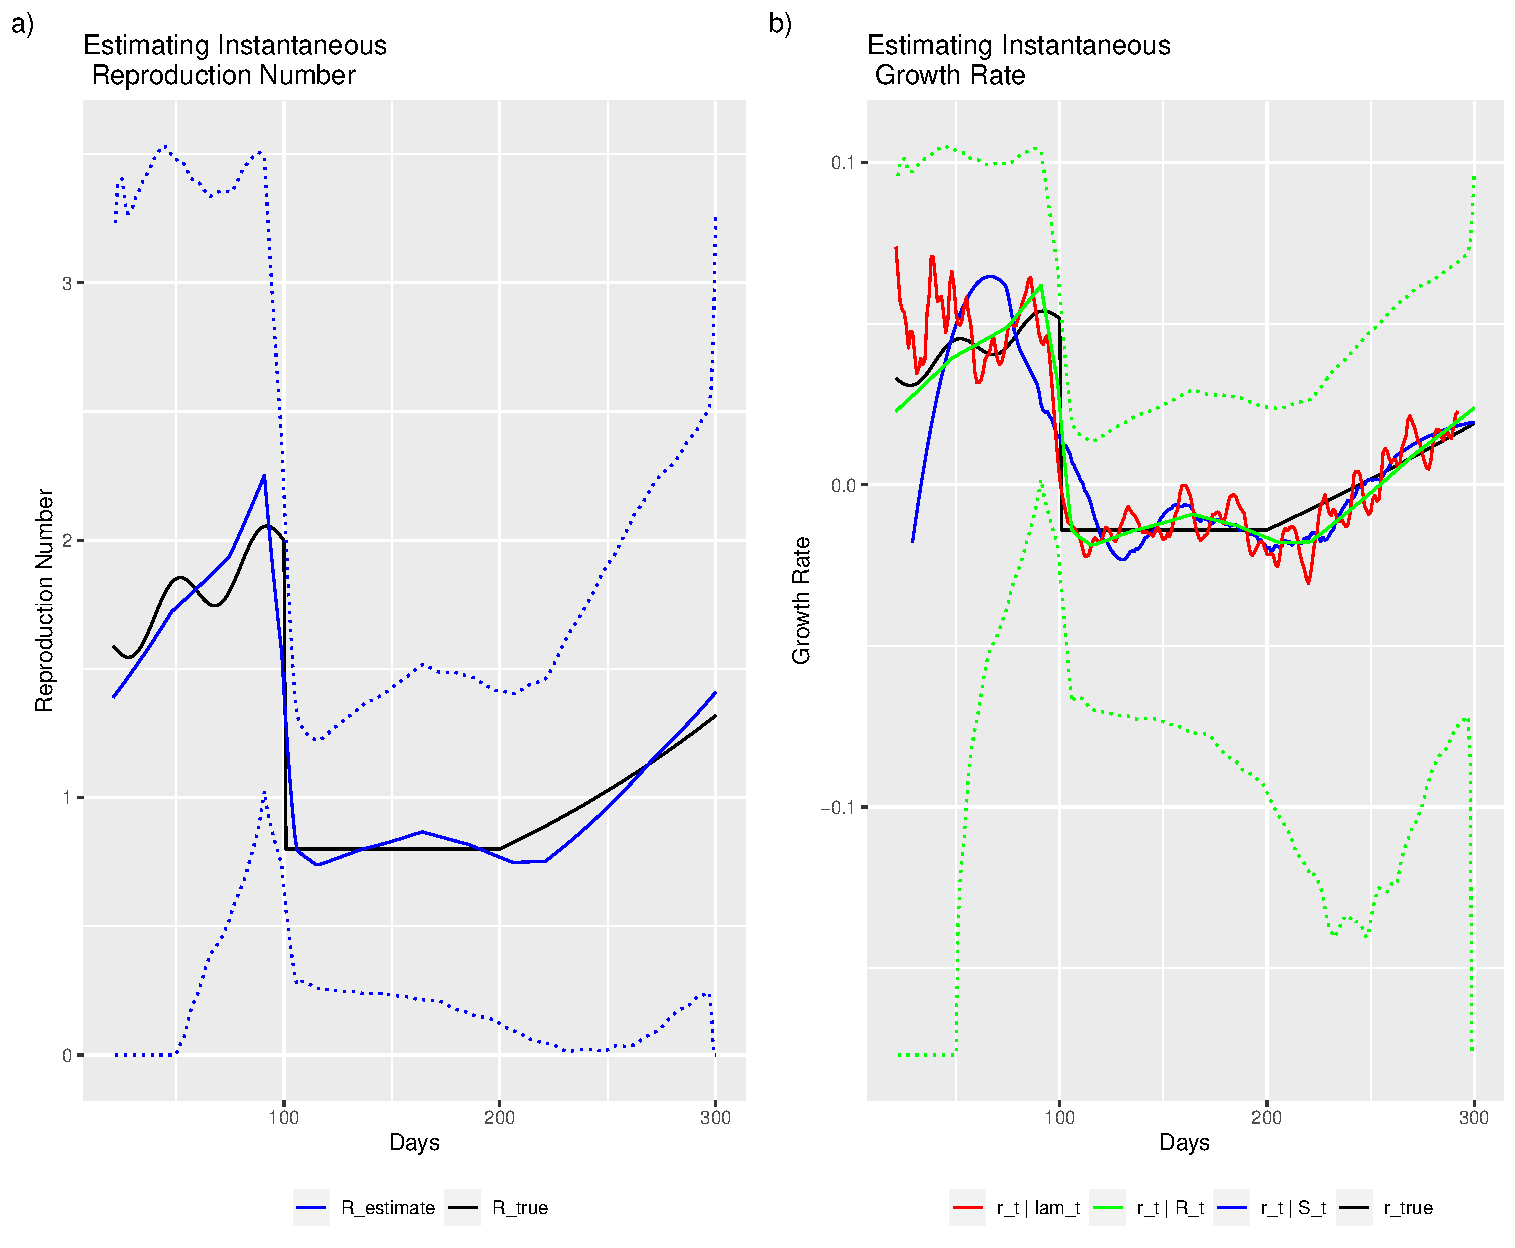
\includegraphics[width = 0.7\textwidth]{weird_fn_1.pdf}
        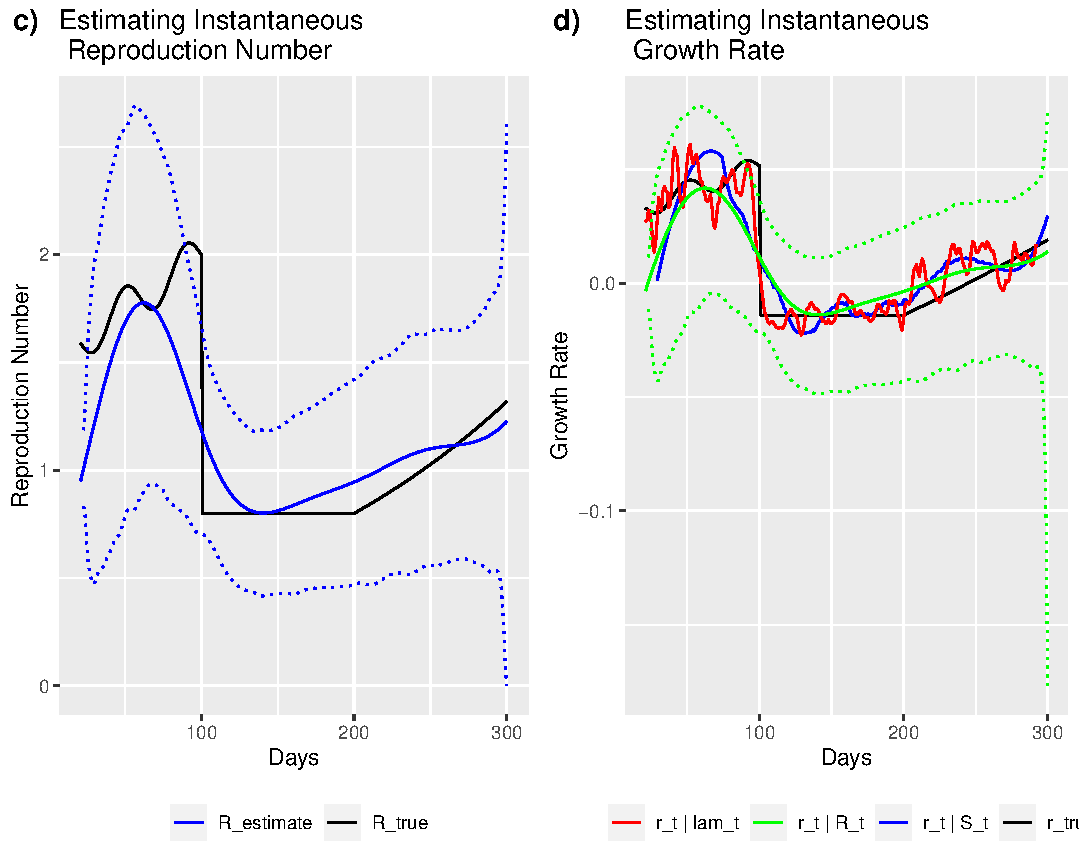
\includegraphics[width = 0.7\linewidth]{weird_fn_3.pdf}
        \caption{asd}
        \label{fig: comp}
      \end{figure}
      



  \section{test}
    We made amazing contributions to the world of musical fractal pasta 
    \citep{McDonald2017,Tibshirani2013}. We use Natbib, so be sure to use
    \citep{Stein1981} for parenthetical references. Or you can say, according to
    \citet{HastieTibshirani2009}, we should strive to balance truth and lies.


\bibliographystyle{rss}
\bibliography{qp.bib}

\end{document}
